\chapter{Nondeterminism, Closure Properties, Regular Expressions}

\section{Nondeterminism}

\begin{eg}\label{eg: NFA}
    This is a nondeterministic finite automaton:\\
    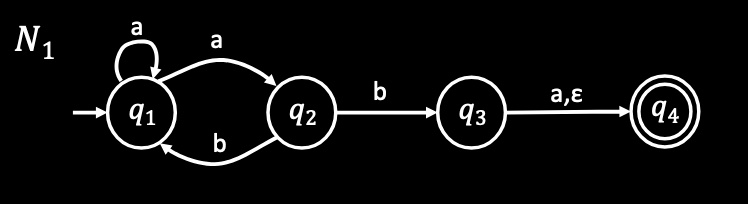
\includegraphics[width=\textwidth]{f2.1.jpg}
    
    What's the difference with what we saw in the last lecture:
    \begin{itemize}
        \item in \(q_1\), when accepting an \(a\), you can either stay in \(q_1\) or go to \(q_2\)
        \item in \(q_1\), if get \(b\) then there's no where to go 
        \item ...
    \end{itemize}

    Example inputs
    \begin{itemize}
        \item ab (accept)
        \item aa (reject)
    \end{itemize}

\end{eg}

New features of nondeterminism:
\begin{itemize}
    \item multiple paths possible (0, 1 or many at each step)
    \item \(\epsilon\)-transition is a "free" move without reading input
    \item Accept input if \underline{some} path leads to accept state (acceptance overrules rejection) (if one of possible ways to go accepts, then accepts)
\end{itemize}

Nondeterminism doesn't correspond to a physical machine we can build, however it is useful mathematically.

\section{NFA}
\begin{definition}
    A \textbf{nondeterministic finite automaton} is a 5-tuple \(Q, \Sigma, \sigma, q_0, F\), where
    \begin{enumerate}
        \item Q is a finite set of states
        \item \(\Sigma\) is a finite alphabet 
        \item \(\sigma: Q \times \Sigma_{\epsilon} \Rightarrow \P(Q)\) is the transition function 
        \item \(q_0 \in Q\) is the start state
        \item \(F \subseteq Q\) is the set of accept states   
    \end{enumerate}  

    In which, \(\Sigma_{\epsilon}\) is a shorthand of \(\Sigma \cup \{ \epsilon \} \).  
    P(Q) means the power set of Q which can be represented as \(P(Q) = {R | R \subseteq Q}\), which is the set which contains all the subset of Q.  
\end{definition}

\begin{eg}
    Check the 
\end{eg}